There are several formulations for the pressure gradient.

\subsection{ config\_pressure\_gradient\_type = 'pressure\_and\_zmid'}
This is the standard setting, and may be used for most configurations.  Here the pressure gradient terms in the momentum equation will have the form
\begin{equation}
\label{ocean:grad p}
- \frac{1}{\rho_0}\nabla_z p = - \frac{1}{\rho_0}\nabla_s p - \frac{\rho g}{\rho_0}\nabla_s z^{mid}.
\end{equation}
where $\nabla_z$ is the horizonal gradient along a constant $z$ surface and $\nabla_s$ is the gradient along a layer, which is a natural way to compute horizontal derivatives within the model.  Note that if a layer's depth is constant in the horizontal, then the second term is zero.

\subsection{ config\_pressure\_gradient\_type = 'Jacobian\_from\_density'}
In this formulation the pressure gradient is rewritten in terms of a sea surface height gradient and the vertical integral of a Jacobian,
\begin{eqnarray}
\label{ocean:grad p Jacobian}
- \frac{1}{\rho_0}\nabla_z p &=& - \frac{\rho_s g}{\rho_0}\nabla_s \zeta - \frac{g}{\rho_0}\int_z^\zeta {\mathcal J}(\rho,z)ds, \\
{\mathcal J}(\rho,z) &=& \left. \frac{\partial \rho}{\partial x} \right|_s \frac{\partial z}{\partial s} 
 - \frac{\partial \rho}{\partial s}  \left. \frac{\partial z}{\partial x} \right|_s 
\end{eqnarray}
where $x$ is a general horizontal direction between two cell centers and $s$ is the vertical coordinate reference, i.e.\ $s$ is constant within a layer.  There are many methods to discretize the Jacobian term.  In the common level method, the density is linearly interpolated or extrapolated within each vertical column to a common level $z_\gamma$ (see Figure \ref{oceanFigure:common level}):
\begin{eqnarray}
- \int_z^\zeta {\mathcal J}(\rho,z)ds &=& \overline{\Delta z} \left( \rho^L - \rho^R \right) \\
\overline{\Delta z} &=& \frac{1}{2} \left(z_2-z_1 + z_4-z_3\right) \\
\rho^L &=& \frac{\rho_1\left(z_2-z_\gamma\right) + \rho_2\left(z_\gamma-z_1\right) }{z_2-z_1}\\
\rho^R &=& \frac{\rho_3\left(z_4-z_\gamma\right) + \rho_4\left(z_\gamma-z_3\right) }{z_4-z_3}\\
z_\gamma &=& \left(1-\gamma\right)z_* + \gamma z_c \\
z_* &=&  \frac{z_4 z_2-z_3z_1}{z_4-z_3 + z_2-z_1} \\
z_c &=&  \frac{z_1+z_2+z_3+z_4}{4} 
\end{eqnarray}
where $z_c$ is the depth for the weighted Jacobian method by \citet{Song98mwr}, and $z_*$ is the depth for the standard Jacobian method, which is the depth of intersection of the diagonals of the trapezoidal element in Figure \ref{oceanFigure:common level}.  Here $\gamma$ weights the choice between these two methods for computing the common level $z_\gamma$.  This formulation for the pressure gradient is described in detail in \citet{Shchepetkin_McWilliams03jgr}, Section 2, method 2, and Section 4.  They found that a coefficient of $\gamma=0.5$, which gives equal weights to the standard and weighted Jacobian methods, minimizes the errors in a seamount test problem.

\begin{figure}[htb]
\centering
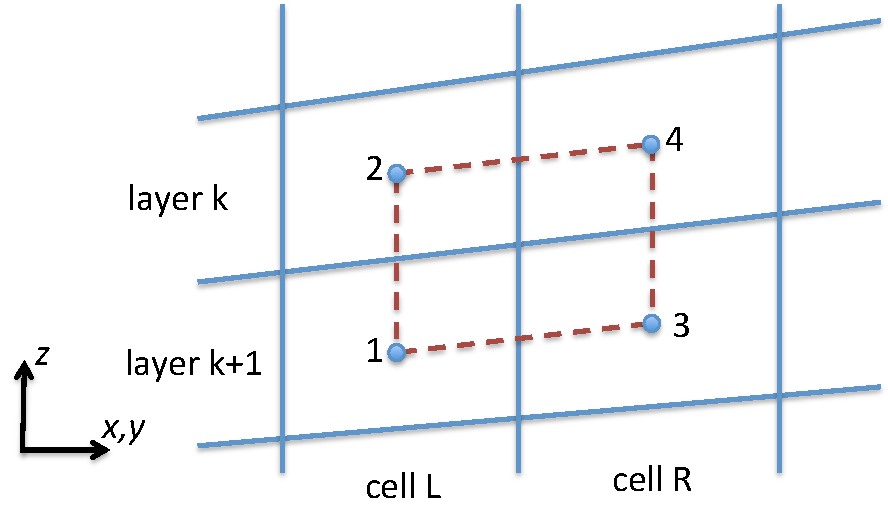
\includegraphics[width=3.5in]{ocean/figures/common_level.pdf}
\caption{Vertical cross-section of ocean grid cells, showing index locations for common level method.  The dots are placed at cell centers in the horizontal and layer mid-depth in the vertical.}
\label{oceanFigure:common level}
\end{figure}

\subsection{ config\_pressure\_gradient\_type = 'Jacobian\_from\_TS'}
This formulation is the same as the previous, except that the Jacobian is computed using a linear expansion in potential temperature and salinity.  This option must be used when layers are extremely tilted, such as with sigma coordinates or under an ice shelf, in combination with a nonlinear equation of state.
\begin{eqnarray}
 {\mathcal J}(\rho,z) &=& -\alpha  {\mathcal J}(\theta,z) + \beta  {\mathcal J}(S,z), 
\end{eqnarray}
where
\begin{eqnarray}
\alpha\left( \theta, S, p\right) &=&  -\left. \frac{\partial \rho}{\partial \theta} \right|_{S,p} \\
\beta\left( \theta, S, p\right) &=&  \left. \frac{\partial \rho}{\partial S} \right|_{\theta,p} 
\end{eqnarray}
are the thermal expansion and saline contraction coefficients, computed at a particular  $\left(\theta, S, p\right)$ by the equation of state \citep[eqn 7.16]{Shchepetkin_McWilliams03jgr}.

\subsection{ config\_pressure\_gradient\_type = 'MontgomeryPotential'}
For isopycnal vertical coordinates, the user may choose to use the Montgomery potential,
\begin{equation}
\label{ocean:Montgomery Potential}
M = \frac{1}{\rho}p+gz
\end{equation}
and replace the pressure terms above with
\begin{equation}
- \nabla_s M.
\end{equation}
See \citet[section 2.1]{Higdon05jcp} for details on the derivation and computation of the Montgomery potential.

% \subsection{ config\_pressure\_gradient\_type = 'MontgomeryPotential\_and\_density'}
% Same as previous, but this formulation includes an extra term,
% \begin{equation}
% - \nabla_s M + p \nabla_s\left(\frac{1}{\rho} \right),
% \end{equation}
% as described by \citet{Bleck02om}, eqn 1 and end of Appendix A.  This formulation has not been extensively tested and is not supported at this time.
